\chapter{Architecture} \label{cpt:architecture}
\section{General overview} \label{sec:classes}
Our project is called ``Lepatriinu'' which is the Estonian word for ``lady
beetle'' (German: ``Marienkäfer'') in order to express our sympathy for Austrian
lady beetles, which are threatened by the superior species of Asian lady
beetles.

Generally the structure of our project is object oriented. Therefore the
functionality is split in several classes. The given framework simple calls
methods which are defined in the package \texttt{at.jku.amp.lepatriinu}.

Additional to the functionality the project comes up with a graphical user
interface which simplifies working on the audio data and represents the results
in a proper fashion.

\begin{figure}[htp]
  \centering
  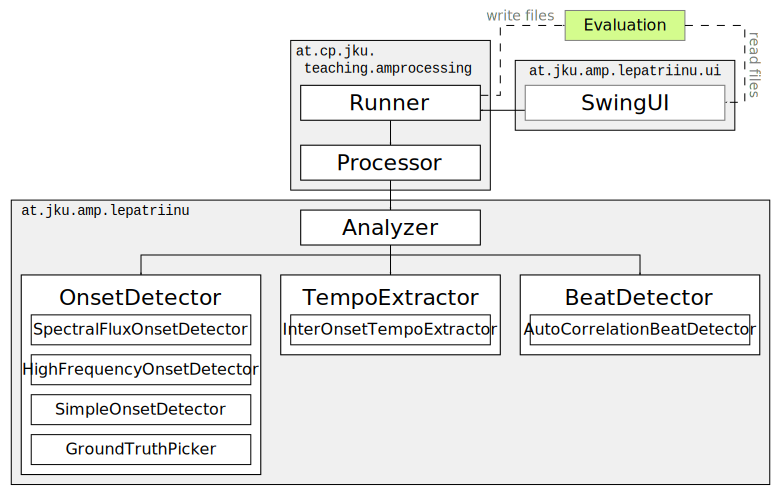
\includegraphics[width=\textwidth-1em]{chapter/ClassDiagram}
  \label{fig:classdiagram}
  \caption{Class diagram}
\end{figure}

%%%%%%%%%%%%%%%%%%%%%%%%%%%%%%%%%%%%%%%%%%%%%%%%%%%%%%%%%%%%%%%%%%%%%%%%%%%%%%%%
% ANALYZER 
%%%%%%%%%%%%%%%%%%%%%%%%%%%%%%%%%%%%%%%%%%%%%%%%%%%%%%%%%%%%%%%%%%%%%%%%%%%%%%%%
\section{\ttfamily Analyzer} \label{sec:analyzer}
The \emph{Analyzer} class defines all the constants that are needed for any
algorithm in the project to succeed. In order to make central configurations
possible, the constants are collected in this single class.

Furthermore it provides the central interface to the
\texttt{at.cp.jku.teaching.am\-pro\-ces\-sing} project. It is initialized with a
pre-processed (e.g. FFT) audio file of type \texttt{Audiofile}. The order of
usage is important. In the first place, onset detection can be done. This
information can directly be retrieved from the audio file. The found onsets are
the base for tempo extraction. Therefore the onset list has to be provided as
parameter of the tempo extraction function. Finally beat detection can be
performed. In order to be able to use the best algorithms both the onset list as
well as the calculated tempo should be provided.

\begin{enumerate}
  \item Onset detection: \texttt{onsets = performOnsetDetection()}
  \item Tempo extraction: \texttt{tempo = performTempoExtraction(onsets)}
  \item Beat Detection: \texttt{beats = performBeatDetection(onsets, tempo)}
\end{enumerate}

%%%%%%%%%%%%%%%%%%%%%%%%%%%%%%%%%%%%%%%%%%%%%%%%%%%%%%%%%%%%%%%%%%%%%%%%%%%%%%%%
% ONSET DETECTION
%%%%%%%%%%%%%%%%%%%%%%%%%%%%%%%%%%%%%%%%%%%%%%%%%%%%%%%%%%%%%%%%%%%%%%%%%%%%%%%%
\section{\ttfamily OnsetDetector} \label{sec:onset}
\emph{OnsetDetector} is the abstract superclass of all onset detection
algorithm's classes. It provides two different peak picking methods which can be
used by any sub class.

\begin{enumerate}
  \item The first peak picking method is taken from lecture slides (5.40) and
  called \emph{Adaptive Thresholding}.
  \item The second one is a slight modification of the adaptive thresholding
  algorithm. Instead of a threshold it simply isolates the highest magnitudes by
  zeroing everything but the peak as well as close neighbors that are lower. As
  a result a clear list of onsets remains. We called this method \emph{mountain
  climbing}.
\end{enumerate}

\subsection*{Constants} \label{ssec:onsetconstants}
\begin{itemize}
  \item \texttt{USE\_MOUNTAIN\_PEAKPICK} defines which peakpicking method to
  use. If constant is \texttt{true}, \emph{mountain peakpicking} is chosen.
  Otherwise \emph{adaptive thresholding} is performed.
  \item \texttt{THRESHOLD\_RANGE} is used to specify the \texttt{int} size of
  the shifted slice used in \emph{adaptive thresholding} as well as the range of
  zeroed neighbors in \emph{mountain climbing}. The best results were produced
  by a range of \texttt{5}.
  \item \texttt{PEAKPICK\_USE\_MEAN} defines whether to use mean
  (\texttt{true}) or median (\texttt{false}) in order to select the threshold
  that is later on applied to all the onset calculations of \emph{adaptive
  thresholding}.
  \item \texttt{THRESHOLD} is used to define a fixed \texttt{int} threshold for
  choosing the magnitude peaks when using \emph{mountain climbing}. The value
  that produced the best results in our experiments was \texttt{13}. 
\end{itemize}

\subsection{\ttfamily SimpleOnsetDetector} \label{ssec:onsetsimple}
This very simplistic method is taken from the given framework. Generally it
calculates the distances between every pair of spectral data bins and validates
it against a fixed threshold of 10.

\subsection{\ttfamily SpectralFluxOnsetDetector} \label{ssec:onsetflux}
This onset detection function implements the idea of spectral differences
(``spectral flux''). Therefore the idea of slide 4.20 was implemented. Because
this method evolved from a copy of \texttt{SimpleOnsetDetector} in the first
place, two minimally different versions of this algorithm were implemented.

The mode can be chosen by the constant \texttt{FLUX\_USE\_TOTAL\_ENERGY}.

\begin{itemize}
  \item \texttt{true}: like the \texttt{SimpleOnsetDetector} the first version
  uses the total energy of each bin in order to calculate the differences, which
  are subsequently processed according to the formula.
  \item \texttt{false}: unlike the first method but according to the slides, the
  second method uses differences of magnitudes between bins. This has the
  unfortunate attitude to need an additional loop.
\end{itemize}

\subsection{\ttfamily HighFrequencyOnsetDetector} \label{ssec:onsethighfreq}
As an alternative to spectral differences the \emph{HighFrequencyOnsetDetector}
implements the idea of so called ``high frequency content'' (slide 4.19). Again
there are two modes that qualify for usage. These can be switched by the
\texttt{boolean} constant \texttt{HIFQ\_USE\_WPHACK}.

\begin{itemize}
  \item \texttt{false}: this mode implements the formula on the slides.
  \item \texttt{true}: unlike the original idea, this mode uses a formula which
  was found on
  Wikipedia\footnote{\url{https://en.wikipedia.org/wiki/High_Frequency_Content}}.
  Essentially the difference is the calculation of the mean, which is performed
  by the formula on the slides but left away in the formula from Wikipedia.
\end{itemize}

\subsection{\ttfamily GroundTruthPicker} \label{ssec:onsetgroundtruth}
We designed the \emph{GroundTruthPicker} just for experimenting with the best
onsets we could possibly get: The original ground truth. It simply reads in the
corresponding ground truth file from the input directory and parses it into a
\texttt{List<Double>}, which it returns. To find the right file we had to expose
the file name in the \texttt{Audiofile}. But as it turned out, the evaluation of
the ground truth isn't even as true as we thought it would be - it was only
considered with an average F-Measure of 92.5\% over all 18 data sets.

%%%%%%%%%%%%%%%%%%%%%%%%%%%%%%%%%%%%%%%%%%%%%%%%%%%%%%%%%%%%%%%%%%%%%%%%%%%%%%%%
% TEMPO EXTRACTION
%%%%%%%%%%%%%%%%%%%%%%%%%%%%%%%%%%%%%%%%%%%%%%%%%%%%%%%%%%%%%%%%%%%%%%%%%%%%%%%%
\section{\ttfamily TempoExtractor} \label{sec:tempo}
\emph{TempoExtractor} is the abstract superclass of which all tempo extractors
should be derived.

\subsection{\ttfamily InterOnsetTempoExtractor} \label{ssec:tempointeronset}
As the name suggests, \emph{InterOnsetTempoExtractor} performs the Inter Onset
Intervals as described in the lecture slides 5.10 through 5.14. The method
calculates the most common gap size between the onsets inside a set of onsets. 

Because of the inaccuracy that evolves when adding vague \texttt{double}
values and the necessity to provide some sort of categorization and
clustering an indirect mapping from the \texttt{double} value of the
gap size to the \texttt{int} value of the number of occurrencies was
established. In order to reach this goal actually two mappings are done:

\begin{enumerate}
  \item \texttt{double} $\rightarrow$ \texttt{int}: specified by the constant
  \texttt{TEMPO\_KEY\_TOLERANCE}, given distances are separated into different
  categories which are consecutively numbered using the \texttt{int} values. To
  be more precise, if \texttt{distance $\pm$ TEMPO\_KEY\_TOLERANCE}
  meets one key in the map, it is put into the same category. Otherwise it is
  put into a new one.
  \item \texttt{int} $\rightarrow$ \texttt{int}: The \emph{value} of the
  mapping in 1 is the \emph{key} of the second mapping, which provides the
  number of occurencies.
\end{enumerate}

Of course this is to be done if the distance is within the range of usual tempi.
Therefore distances that are smaller than \texttt{MIN\_TEMPO} or greater than
\texttt{MAX\_TEMPO} are not taken into account.

The tempo then is returned in \emph{beats per minute} (bpm).

%%%%%%%%%%%%%%%%%%%%%%%%%%%%%%%%%%%%%%%%%%%%%%%%%%%%%%%%%%%%%%%%%%%%%%%%%%%%%%%%
% BEAT DETECTION
%%%%%%%%%%%%%%%%%%%%%%%%%%%%%%%%%%%%%%%%%%%%%%%%%%%%%%%%%%%%%%%%%%%%%%%%%%%%%%%%
\section{\ttfamily BeatDetector} \label{sec:beat}
Also \emph{BeatDetector} is an abstract class, thats purpose is to be the
superclass of all beat detection algorithms. 

\subsection{\ttfamily AutoCorrelationBeatDetector} \label{ssec:beatauto}
This subclass implements beat detection based on auto correlation. It
accommodates an enumeration, named \emph{Mode}, which allows to switch between
three different ideas and implementations:

\begin{enumerate}
  \item \texttt{AUTO\_TEMPO\_CORRELATION} simply implements the idea of the
  pulse train, described on slides 5.15 through 5.19. To tackle the inaccuracy the
  list of onsets will always carry along we use a threshold, called
  \texttt{AUTO\_PHASE\_TOLERANCE} which, after excessive testing we found best
  to be set around 0.21 and pushed it up to 48\% (average over all 18 provided data
  sets).
  \item \texttt{AUTO\_ONSET\_CORRELATION} represents the implementation of the
  IOI idea presented on lecture slides 5.10 through 5.14.
  \item \texttt{AUTO\_SPECTRAL\_CORRELATION} was the attempt to improve the
  onset correlation by trying to reinterpret the formulas as to be the spectral data
  instead of the onsets. It didn't work out that well (less than 4\% over 18
  data sets).
\end{enumerate}

%%%%%%%%%%%%%%%%%%%%%%%%%%%%%%%%%%%%%%%%%%%%%%%%%%%%%%%%%%%%%%%%%%%%%%%%%%%%%%%%
% BEST RESULTS
%%%%%%%%%%%%%%%%%%%%%%%%%%%%%%%%%%%%%%%%%%%%%%%%%%%%%%%%%%%%%%%%%%%%%%%%%%%%%%%%
\section{Best practices} \label{sec:bestresults}
The best results were reached by using the following configuration:

\begin{itemize}
  \item Onset detection:
  \begin{itemize}
    \item onset detector: \texttt{SpectralFluxOnsetDetector} (see
    \ref{ssec:onsetflux})
    \item mode: \texttt{USE\_TOTAL\_ENERGY = true}
    \item peak picking: \texttt{USE\_MOUNTAIN\_PEAKPICK = true} (see
    \ref{sec:onset})
    \item constants: \texttt{THRESHOLD = 13} and \texttt{THRESHOLD\_RANGE = 5}
  \end{itemize}
  \item Tempo extraction:
  \begin{itemize}
    \item tempo extractor: \texttt{InterOnsetTempoExtractor} (see
    \ref{ssec:tempointeronset})
    \item constants: \texttt{MIN\_TEMPO = 0.3} (= 200 bpm), \texttt{MAX\_TEMPO =
    1} (= 60 bpm) and \texttt{TEMPO\_KEY\_TOLERANCE = 0.0195}.
  \end{itemize}
  \item Beat detection:
  \begin{itemize}
    \item beat detector: \texttt{AutoCorrelationBeatDetector} (see
    \ref{ssec:beatauto})
    \item mode: \texttt{AUTO\_FUNCTION = AUTO\_TEMPO\_CORRELATION}
    \item constant: \texttt{AUTO\_PHASE\_TOLERANCE = 0.21}
  \end{itemize}
\end{itemize}